\documentclass[../main.tex]{subfiles}
\begin{document}
    \chapter{Research Method}\label{chap:research_method}
    %This section will contain:
    %TODO: Explain the used method. %TODO research method
    %TODO: Hypothese/research questions %TODO research question
    $<<$ Introduction of this chapter $>>$
    
    \section{Types}
    Explain here what I mean with a type...
    
    \subsection{PHP types}
    PHP has a similar class inheritance structure and interface implementation as Java.
    The difference is that in PHP all class are $public$, and no inner classes are allowed. 
    \\
    The basis types in PHP are integers, floats (similar to doubles and reals), booleans, strings, arrays, resources and null.
    When variables are initialised without a values, they are null. The recourse type is a special one which is not important for this research.
  

  
    \Blindtext
    
    \subsection{Subtypes}
    The subtype relation of class inheritance is a \gls{transitive closure} relation.
    A class extension of class A on class B will define class A as a subtype of class B.
    If class B has no extension, then class B will be a subtype of object().
    This means that every class is a subtype of object().
    
    
    \begin{wrapfigure}{r}{0.5\textwidth}
    \centering
    \begin{subfigure}{.25\textwidth}
      \centering
      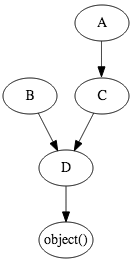
\includegraphics[scale=0.5]{img/subtype}
      \caption{Inheritance relation}
      \label{fig:subtype}
    \end{subfigure}%
    \begin{subfigure}{.25\textwidth}
      \centering
      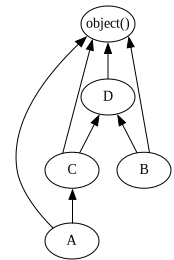
\includegraphics[scale=0.5]{img/subtype_tc}
      \caption{Subtype relation}
      \label{subtype_tc}
    \end{subfigure}
    \caption{Relation of subtypes among classes}
    \label{fig:subtypes}
    \end{wrapfigure}
    
    \lstinputlisting[language=PHP,label=assignment1,caption=Inheritance in PHP]{src/php/inheritance.php}



    
    \section{Constraint extraction}
       
    Introduction is needed here... for now I will just list the types that I have found.
    Maybe this needs to be moved to a different chapter.
    \\
    This is a list of items which are not supported yet:

    \begin{itemize}
        \item Assign statements:
        \begin{itemize}
            \item Ref assign :: $\$a \; = \; \&\$b$
            \item List assign :: $list(\$a, \$b) = array("one", "two");$
        \end{itemize}
        
        \item References (in PHP they are symbol table aliases)
        \begin{itemize}
            \item on expression assignments :: $\$a \; = \; \&\$b$
            \item on functions :: function $\&f()$ $\{ \dots \}$
            \item on parameters :: function $f(\$a)$ $\{ \dots \}$             
        \end{itemize}

        \item Variable structures:
        \begin{itemize}
            \item Variable variables :: $\$\$a;$
            \item \sout{Variable class instantiation} :: $new \; \$a;$
            \item \sout{Variable method or function calls} :: $\$a();$
        \end{itemize}
        
        \item Method or function parameters (including type hints)
        
        \item Casts of expressions
        
        
    \end{itemize}

    \hrulefill
    \\
    Note to myself ::
    \\
    type has field \\
    type has name \\
    type has method \\
    type has magic method \\
    
    \hrulefill

    \begin{prooftree}
        \AxiomC{$E_1 = E_2$}
        \UnaryInfC{$[E_2]<:[E_1]$}
    \end{prooftree}
    \lstinputlisting[language=PHP,label=assignment1,caption=Assignment]{src/php/assignment1.php}
    \hrulefill

    \lstinputlisting[language=PHP,label=assignment2,caption=Assignments with operators resulting in ints]{src/php/assignment2.php}
    \begin{prooftree}
        \AxiomC{
        ($E_1$ $\&=$ $E_2$) $\lor$
        ($E_1$ $\vert=$ $E_2$) $\lor$
        $E_1$ \^{}= $E_2$) $\lor$
        ($E_1$ $<<=$ $E_2$) $\lor$
        ($E_1$ $>>=$ $E_2$) $\lor$
        ($E_1$ $\%=$ $E_2$)
        }
        \UnaryInfC{$[E_1] = int()$}
    \end{prooftree}
    \hrulefill

    \lstinputlisting[language=PHP,label=assignment3,caption=Assignments with string concat operator]{src/php/assignment3.php}    
    \begin{prooftree}
        \AxiomC{$E_1$ .= $E_2$}
        \UnaryInfC{$[E_1] = string()$}
    \end{prooftree}    
    \hrulefill
    
    \lstinputlisting[language=PHP,label=assignment4,caption=Assignments with operators]{src/php/assignment4.php}
    \begin{prooftree}
        \AxiomC{
        ($E_1$ $/= E_2$) $\lor$
        ($E_1 -= E_2$)
        }
        \UnaryInfC{$[E_1] = int()$}
    \end{prooftree}    
    \hrulefill
            
    \lstinputlisting[language=PHP,label=assignment5,caption=Assignments with operators]{src/php/assignment5.php}
    \begin{prooftree}
        \AxiomC{
        ($E_1$ *= $E_2$) $\lor$
        ($E_1$ += $E_2$)
        }
        \UnaryInfC{$[E_1] <: int()$}
    \end{prooftree}    
    \hrulefill
    
    \lstinputlisting[language=PHP,label=comparisonOperators.php,caption=Comparison operators]{src/php/comparisonOperators.php}
    \begin{prooftree}
        \AxiomC{
        ($E_1$ $==$ $E_2$) $\lor$
        ($E_1$ $===$ $E_2$) $\lor$
        ($E_1$ $!=$ $E_2$) $\lor$
        ($E_1$ $<>$ $E_2$) $\lor$
        ($E_1$ $!==$ $E_2$)
        $\subseteq E$
        }
        \UnaryInfC{$[E] = bool()$}
    \end{prooftree}    
    \begin{prooftree}
        \AxiomC{
        ($E_1$ $<$ $E_2$) $\lor$
        ($E_1$ $>$ $E_2$) $\lor$
        ($E_1$ $<=$ $E_2$) $\lor$
        ($E_1$ $>=$ $E_2$)
        $\subseteq E$
        }
        \UnaryInfC{$[E] = bool()$}
    \end{prooftree}    
    \hrulefill

   \lstinputlisting[language=PHP,label=instantiation1,caption=Class instantiation]{src/php/instantiation1.php}
    \begin{prooftree}
        \AxiomC{
        $new \; C$
        $\subseteq \Gamma$
        }
        \AxiomC{
        $class \; C$()* ${ \dots }$
        $\subseteq \Gamma$
        }
        \BinaryInfC{$[new \; C] = C, C.name == [new \; C].name$}
    \end{prooftree}
    *no required params in constructor \\
    \hrule    
     
    \lstinputlisting[language=PHP,label=instantiation2,caption=Class instantiation with parameters]{src/php/instantiation2.php}
    \begin{prooftree}
        \AxiomC{
        $new \; C$ ($E_1$, $E_2$, $\dots$, $E_k$)
        $\subseteq \Gamma$
        }
        \AxiomC{
        $class \; C$ ($th_1$ $E_1$, $th_2$ $E_2$, $\dots$, $th_k$ $E_k$)
        $\subseteq \Gamma$
        }
        \BinaryInfC{$[new \; C] = C, C.name == [new \; C].name$}
    \end{prooftree}
    // todo: add something about the parameter constraints (note to myself: misschien moeten deze 'los' behandeld worden.) \\
    // th = typeHint \\
    \hrule  
    
        \lstinputlisting[language=PHP,label=instantiation3,caption=Class instantiation of an expression]{src/php/instantiation3.php}
    \begin{prooftree}
        \AxiomC{
        $new \; E_1$
        $\subseteq \Gamma$
        }
        \UnaryInfC{$[new \; E_1]$ = object()}
    \end{prooftree}
    \hrule  

    \lstinputlisting[language=PHP,label=function1,caption=Type of variable within their scope; this applies to global- function- and method- scope]{src/php/function1.php}
    \begin{prooftree}
        \AxiomC{
        $E, E', E'', E''' \dots \; etc$
        $\subseteq f$
        }
        \UnaryInfC{$[E] = [E] \lor [E'] \lor [E''] \lor [E'''] \dots \; etc$}
    \end{prooftree}    
    \hrulefill
    
    \lstinputlisting[language=PHP,label=return1,caption=No return statements in function or method]{src/php/return1.php}
    \begin{prooftree}
        \AxiomC{
        return
        $\not \subseteq f$
        }
        \UnaryInfC{$[f] = null()$}
    \end{prooftree}    
    \hrulefill
                  
    \lstinputlisting[language=PHP,label=return2,caption=Return of a function or method; every exit path ends with a return statement]{src/php/return2.php}
    \begin{prooftree}
        \AxiomC{
        (return $E_1$) $\lor$
        (return $E_2$) $\lor$
        $\cdots$ $\lor$
        (return $E_k$)
        $\subseteq f$
        }
        \UnaryInfC{$[f] <: [E_1] \lor [E_2] \lor \cdots \lor [E_k]$}
    \end{prooftree}    
    \hrulefill
    
    \lstinputlisting[language=PHP,label=return3,caption=Return with possible no return value]{src/php/return3.php}
    \begin{prooftree}
        \AxiomC{
        (return $E_1$) $\lor$
        (return $E_2$) $\lor$
        $\cdots$ $\lor$
        (return $E_k$) $\lor$
        ($\neg$ return)
        $\subseteq f$
        }
        \UnaryInfC{$[f] <: [E_1] \lor [E_2] \lor \cdots \lor [E_k] \lor null() $}
    \end{prooftree}    
    \hrulefill
        
    \lstinputlisting[language=PHP,label=functionCall1,caption=Functional call]{src/php/functionCall1.php}
    \begin{prooftree}
        \AxiomC{
        $f()$
        $\subseteq \Gamma$
        }
        \UnaryInfC{$[f()] <:$ return of $[f]$}
    \end{prooftree}    
    \hrulefill
         
    \lstinputlisting[language=PHP,label=functionCall2,caption=Variable function call]{src/php/functionCall2.php}
    \begin{prooftree}
        \AxiomC{
        $E_1()$ $\subseteq \Gamma$
        }
        \UnaryInfC{$[E_1()] = mixed()$}
    \end{prooftree}    
    \hrulefill
    
    How to resolve expressions:
    \begin{itemize}
        \item Find all expressions which are defined above and annotate them with @type.
        \item Annotate the rest of the expressions with @type = any();
    \end{itemize}

       
    
    \section{Annotations}
    Explain how the annotations are added to the constraints.
    \Blindtext
    
    \section{Constraint solving}
    Explain what will be done to solve the constraints.
    \\
    \Blindtext
    
    \section{Case Study}
    Explain how the case study is performed.
    \\
    \Blindtext

\end{document}
